\documentclass[11pt,a4paper]{article}

% --- Langue & encodage (pdfLaTeX) ---
\usepackage[T1]{fontenc}
\usepackage[utf8]{inputenc}
\usepackage[french]{babel}
\usepackage{listings}  % Pour les blocs de code
\usepackage{xcolor}    % Pour la coloration syntaxique
\usepackage{float}  % Pour le [H]
\usepackage{amsmath}
\usepackage{amssymb}
\usepackage{listingsutf8}

% Configuration optionnelle pour les listings
\lstset{
  inputencoding=utf8,
  language=Python,
  basicstyle=\ttfamily\small,
  numbers=left,
  numberstyle=\tiny,
  showstringspaces=false,
  breaklines=true,
  upquote=true
}

\lstset{literate=
  {é}{{\'e}}1 {è}{{\`e}}1 {ê}{{\^e}}1 {ë}{{\"e}}1
  {à}{{\`a}}1 {ù}{{\`u}}1 {ç}{{\c c}}1
  {É}{{\'E}}1 {È}{{\`E}}1 {À}{{\`A}}1
}

% --- Mise en page & utilitaires ---
\usepackage[margin=2.5cm]{geometry}
\usepackage{graphicx}    % pour \includegraphics
\usepackage[hidelinks]{hyperref}

\begin{document}

% =============================
% Page de garde
% =============================
\begin{titlepage}
    \centering

    % Logo université (facultatif : commente la ligne si l'image n'existe pas)
    % Place l'image ici : images/logo.png
    
\includegraphics[width=0.25\textwidth]{images/logo.png}\par\vspace{1cm}

    {\scshape\LARGE Université de Montpellier \par}
    {\scshape Faculté des Sciences\par}
    {\scshape Recherches Mathématiques\par}
    \vspace{1.5cm}

    % Titre
    {\Huge \bfseries HAX907X - Apprentissage statistique \par}
    \vspace{0.5cm}
    {\Large M2 SSD--BIOSTAT\par}
    \vspace{1cm}

    \rule{\linewidth}{0.5pt}\\[0.4cm]
    {\huge \itshape Support Vector Machines (SVM)\par}
    \rule{\linewidth}{0.5pt}\\[2cm]

    % Auteur
    \begin{center}
    \textbf{Réalisé par :}\\
  Achiq Aya
\end{center}


    \vfill

    % Date
    {\large 03 octobre 2025\par}
\end{titlepage}

\tableofcontents
\newpage

% --- Décommente UNE des deux options ci-dessous ---

\section{Introduction}
Ce TP s’inscrit dans le cadre du cours d’Apprentissage Statistique et a pour objectif de mettre en pratique les méthodes de classification par Support Vector Machine (SVM). Les SVM sont des algorithmes puissants et largement utilisés, car ils permettent de séparer efficacement des données en classes, aussi bien dans des situations simples (données linéairement séparables) que dans des contextes plus complexes grâce à l’utilisation de noyaux.

L’idée générale d’un SVM est de trouver un hyperplan qui sépare au mieux les différentes classes, en maximisant la marge entre elles. Certains points de données, appelés vecteurs supports, jouent un rôle essentiel car ils déterminent la position de cet hyperplan. L’algorithme peut aussi être adapté grâce à des paramètres comme le coefficient de régularisation (C) ou le choix du noyau (linéaire, polynomial, gaussien, etc.) qui modifient sa flexibilité et sa capacité à s’adapter aux données.

Au fil de ce TP, nous allons explorer plusieurs aspects pratiques des SVM. Nous commencerons par une classification simple sur le jeu de données Iris, puis nous étudierons l’impact du noyau et du paramètre C dans des situations plus délicates, comme lorsque les classes sont déséquilibrées. Enfin, nous appliquerons les SVM à un problème plus réaliste de reconnaissance de visages, où l’on verra également l’intérêt de techniques complémentaires comme la réduction de dimension par ACP (PCA).

L’objectif est donc à la fois de comprendre le principe des SVM et de voir concrètement comment leur performance dépend du choix des paramètres et des données utilisées.

\section{Principes et fondements des SVM}

\subsection{Problème de classification binaire}
En classification supervisée, on dispose d’un ensemble de données d’apprentissage :
\[
D_n = \{(x_i, y_i)\}_{i=1}^n, \quad x_i \in \mathbb{R}^p, \; y_i \in \{-1, +1\}.
\]
Chaque observation $x_i$ est décrite par $p$ variables, et $y_i$ est son étiquette (classe).
L’objectif est de construire une fonction de prédiction
\[
\hat{f} : \mathbb{R}^p \to \{-1, +1\},
\]
capable de classer correctement de nouveaux exemples.

\subsection{Hyperplan et marge maximale}
Un classifieur linéaire sépare l’espace à l’aide d’un hyperplan :
\[
f(x) = \text{sign}(\langle w, x \rangle + b),
\]
où $w$ est un vecteur normal au plan et $b$ un biais.
L’idée clé des SVM est de trouver l’hyperplan qui \textbf{maximise la marge}, c’est-à-dire la distance entre le plan et les points les plus proches des deux classes.
Ces points particuliers sont appelés \textit{vecteurs supports}, car ce sont eux qui déterminent la position finale de l’hyperplan optimal.

\subsection{Formulation d’optimisation}
Dans le cas idéal où les classes sont parfaitement séparables, la contrainte est :
\[
y_i(\langle w, x_i \rangle + b) \ge 1 \quad \forall i.
\]
Maximiser la marge revient alors à résoudre :
\[
\min_{w,b} \frac{1}{2}\|w\|^2.
\]

En pratique, les données ne sont pas toujours séparables. On introduit alors des variables de relaxation $\xi_i \ge 0$ qui autorisent des erreurs, avec une pénalisation dans la fonction objectif :
\[
\min_{w,b,\xi} \frac{1}{2}\|w\|^2 + C \sum_{i=1}^n \xi_i,
\]
sous les contraintes
\[
y_i(\langle w, x_i \rangle + b) \ge 1 - \xi_i, \quad \xi_i \ge 0.
\]
Le paramètre $C$ règle le compromis entre \textbf{large marge} (modèle simple, tolérant aux erreurs) et \textbf{faible erreur d’entraînement} (modèle plus complexe).

\subsection{Problème dual et vecteurs supports}
À l’aide des multiplicateurs de Lagrange, le problème se reformule sous forme duale :
\[
\max_{\alpha} \sum_{i=1}^n \alpha_i - \frac{1}{2}\sum_{i,j=1}^n \alpha_i \alpha_j y_i y_j K(x_i, x_j),
\]
avec $0 \le \alpha_i \le C$ et $\sum_{i=1}^n \alpha_i y_i = 0$.

La solution optimale s’écrit comme combinaison linéaire des vecteurs supports :
\[
w^* = \sum_{i=1}^n \alpha_i^* y_i \Phi(x_i).
\]
Seuls les points avec $\alpha_i > 0$ (vecteurs supports) influencent réellement la décision.

\subsection{Noyaux et \textit{kernel trick}}
Pour traiter des cas non linéaires, on projette les données via une transformation
\[
\Phi : \mathbb{R}^p \to H
\]
dans un espace de caractéristiques $H$ de grande dimension.
Le classifieur reste linéaire dans $H$, mais devient non linéaire dans l’espace initial.

Grâce au \textit{kernel trick}, il n’est pas nécessaire de calculer $\Phi(x)$ explicitement :
il suffit d’utiliser une fonction noyau $K$ vérifiant
\[
K(x, x') = \langle \Phi(x), \Phi(x') \rangle.
\]

Les noyaux les plus courants sont :
\begin{itemize}
    \item \textbf{Linéaire} : $K(x,x') = \langle x, x' \rangle$
    \item \textbf{Gaussien RBF} : $K(x,x') = \exp(-\gamma \|x - x'\|^2)$
    \item \textbf{Polynôme} : $K(x,x') = (\alpha + \beta \langle x, x' \rangle)^\delta$
\end{itemize}

\subsection{Extension au multi-classe}
Les SVM sont conçus pour la classification binaire. Pour les problèmes à $K > 2$ classes, on utilise des stratégies d’assemblage :
\begin{itemize}
    \item \textbf{Un-contre-tous (One-vs-Rest)} : on entraîne $K$ classifieurs, chacun séparant une classe contre toutes les autres.
    \item \textbf{Un-contre-un (One-vs-One)} : on entraîne un classifieur pour chaque paire de classes, soit $K(K-1)/2$ modèles.
    La prédiction finale repose sur un vote majoritaire.
\end{itemize}

Ces approches sont intégrées dans des bibliothèques comme \textit{scikit-learn}.


\section{Classification sur le dataset Iris}

\subsection{Présentation des données}

On utilise le jeu de données Iris qui contient des mesures sur trois espèces de fleurs. Pour ce TP, on se limite à une classification binaire entre deux espèces (Versicolor et Virginica) en ne gardant que les deux premières variables. Cette simplification permet de visualiser facilement les résultats dans un espace bidimensionnel.

Les données ont d'abord été standardisées (moyenne nulle, écart-type unitaire) pour que toutes les variables soient sur la même échelle, ce qui est important pour les SVM. On a ensuite divisé le jeu en deux parties égales : 50\% pour l'entraînement et 50\% pour le test.

\subsection{Classification avec noyau linéaire}

On commence par tester un SVM avec noyau linéaire. L'idée est de trouver la meilleure valeur du paramètre de régularisation $C$ qui contrôle le compromis entre marge large et erreurs d'entraînement. Pour cela, on utilise une validation croisée à 5 plis et on teste 200 valeurs de $C$ entre $10^{-3}$ et $10^3$.

\begin{lstlisting}[language=Python, caption=Optimisation du paramètre C avec noyau linéaire]
parameters = {'kernel': ['linear'], 
              'C': list(np.logspace(-3, 3, 200))}
clf_linear = GridSearchCV(SVC(), parameters, cv=5)
clf_linear.fit(X_train, y_train)
\end{lstlisting}

\textbf{Résultats :}
\begin{itemize}
    \item Meilleur $C$ : 0.297
    \item Score train : 66\%
    \item Score test : 66\%
\end{itemize}

Le fait que les scores d'entraînement et de test soient identiques est plutôt bon signe : le modèle ne surapprend pas. Par contre, 66\% de précision reste modeste, ce qui signifie qu'un tiers des exemples sont mal classés. On voit sur la visualisation que la frontière linéaire ne peut pas parfaitement séparer les deux classes qui se chevauchent naturellement.

\subsection{Comparaison avec un noyau polynomial}

Pour essayer d'améliorer les résultats, on teste un noyau polynomial qui peut capturer des relations non linéaires. On fait varier trois paramètres : $C$, le degré du polynôme et $\gamma$ qui contrôle la complexité du noyau.

\begin{lstlisting}[language=Python, caption=Optimisation avec noyau polynomial]
Cs = list(np.logspace(-3, 3, 5))
gammas = 10. ** np.arange(1, 2)
degrees = np.r_[1, 2, 3]

parameters = {'kernel': ['poly'], 
              'C': Cs, 
              'gamma': gammas, 
              'degree': degrees}
clf_poly = GridSearchCV(SVC(), parameters, cv=5)
clf_poly.fit(X_train, y_train)
\end{lstlisting}

\textbf{Résultats :}
\begin{itemize}
    \item Meilleurs paramètres : $C = 0.0316$, degré = 1, $\gamma = 10.0$
    \item Score train : 66\%
    \item Score test : 66\%
\end{itemize}

L'optimisation par validation croisée a exploré différents degrés polynomiaux (1, 2, 3) ainsi que diverses valeurs de $C$ et $\gamma$. Le fait que le degré optimal soit 1 signifie que le noyau polynomial se comporte exactement comme un noyau linéaire dans ce cas, car :
\[
K(x,x') = (10.0 \times \langle x, x' \rangle)^1 = 10.0 \times \langle x, x' \rangle
\]

Ceci suggère que la relation entre les deux variables n'est pas fondamentalement non-linéaire, ou que le chevauchement naturel entre les deux espèces ne peut être résolu par une complexification du modèle.

\subsection{Visualisation des frontières}

La figure ci-dessous montre les données et les frontières de décision trouvées par les deux modèles.

\begin{figure}[H]
\centering
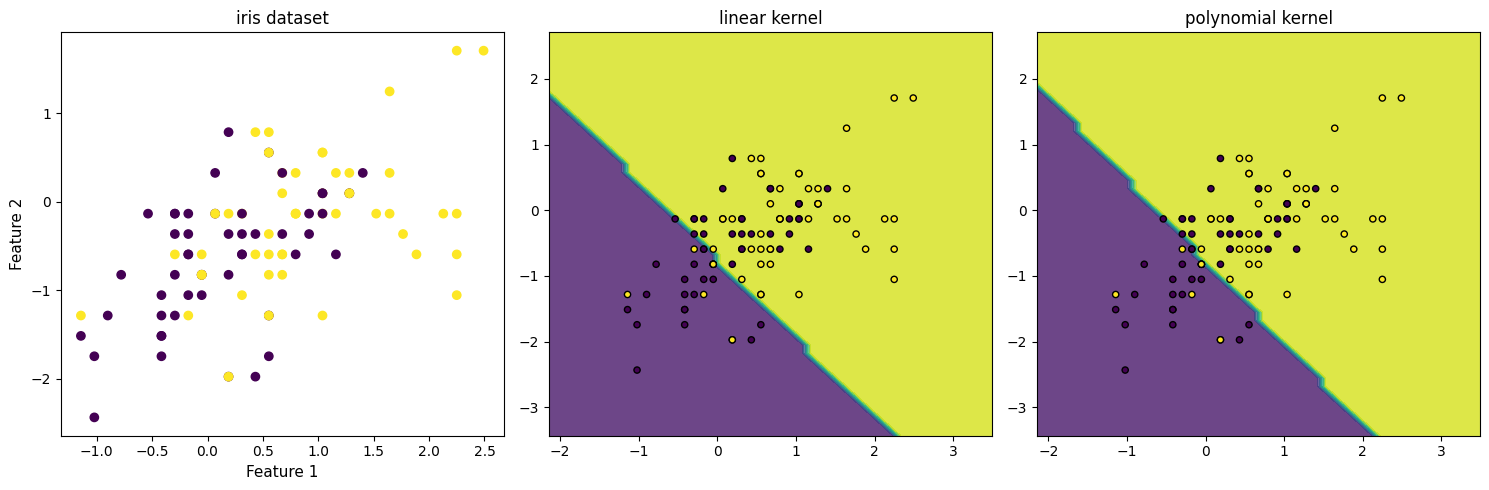
\includegraphics[width=\textwidth]{images/iris_classification.png}
\caption{Classification du dataset Iris avec noyaux linéaire et polynomial}
\end{figure}

On remarque que les deux frontières sont presque superposables, ce qui confirme que le noyau polynomial n'apporte pas d'amélioration ici. Les points mal classés se situent surtout dans la zone où les deux classes se mélangent.

\subsection{Analyse comparative et discussion}

Le tableau suivant résume les performances obtenues avec les différents noyaux testés :

\begin{table}[h]
\centering
\begin{tabular}{|l|c|c|c|}
\hline
\textbf{Noyau} & \textbf{Paramètres optimaux} & \textbf{Score train} & \textbf{Score test} \\
\hline
Linéaire & $C = 0.297$ & 66\% & 66\% \\
\hline
Polynomial & $C = 0.0316$, degré = 1, $\gamma = 10.0$ & 66\% & 66\% \\
\hline
\end{tabular}
\caption{Comparaison des performances selon le noyau}
\end{table}

La précision de 66\% peut sembler modeste, mais elle s'explique par plusieurs facteurs. Premièrement, nous n'utilisons que deux variables sur les quatre disponibles, ce qui limite l'information accessible au modèle. Deuxièmement, les classes Versicolor et Virginica présentent un chevauchement naturel dans l'espace des deux premières variables, rendant une séparation parfaite impossible. 

L'égalité entre les scores train et test (66\% dans les deux cas) est toutefois positive : elle indique que le modèle généralise correctement sans sur-apprentissage ni sous-apprentissage. Le paramètre $C$ optimal relativement faible ($C = 0.297$ pour le linéaire) suggère qu'une régularisation modérée est préférable, favorisant une marge plus large plutôt qu'une classification parfaite des données d'entraînement.

Le fait que la validation croisée ait sélectionné un noyau polynomial de degré 1 (équivalent à un noyau linéaire) confirme que l'ajout de non-linéarité n'est pas bénéfique pour ce problème particulier. 
Cela peut être dû soit à la nature intrinsèquement linéaire de la séparation entre ces deux espèces dans l'espace considéré, soit au fait que le chevauchement des classes est tel qu'aucun modèle ne peut significativement améliorer les performances au-delà de 66\%.

\section{Classification de visages}

\subsection{Présentation du problème et préparation des données}

On travaille maintenant sur un problème de reconnaissance de visages à partir du dataset LFW (Labeled Faces in the Wild). L'objectif est de distinguer deux personnalités politiques : Tony Blair et Colin Powell. 

Chaque image est convertie en niveaux de gris en calculant la moyenne des trois canaux de couleur. Chaque pixel devient ensuite une variable, ce qui génère un espace de très haute dimension (plusieurs milliers de variables pour quelques centaines d'exemples). Les données sont standardisées pixel par pixel avant l'apprentissage.

\begin{lstlisting}[language=Python, caption=Extraction des caractéristiques et standardisation]
# Conversion en niveaux de gris et vectorisation
X = (np.mean(images, axis=3)).reshape(n_samples, -1)

# Standardisation
X -= np.mean(X, axis=0)
X /= np.std(X, axis=0)
\end{lstlisting}

Le jeu de données est divisé en deux moitiés égales par permutation aléatoire des indices, garantissant ainsi une répartition non biaisée entre ensemble d'entraînement et ensemble de test.

\subsection{Influence du paramètre de régularisation C}

Pour comprendre l'impact de $C$, on a entraîné des SVM avec noyau linéaire pour 11 valeurs de $C$ allant de $10^{-5}$ à $10^5$ sur une échelle logarithmique.

\begin{lstlisting}[language=Python, caption=Recherche du meilleur paramètre C]
Cs = 10. ** np.arange(-5, 6)
scores = []

for C in Cs:
    clf = SVC(kernel='linear', C=C)
    clf.fit(X_train, y_train)
    y_pred = clf.predict(X_test)
    scores.append(accuracy_score(y_test, y_pred))

ind = np.argmax(scores)
print("Best C: {}".format(Cs[ind]))
\end{lstlisting}

\begin{figure}[H]
\centering
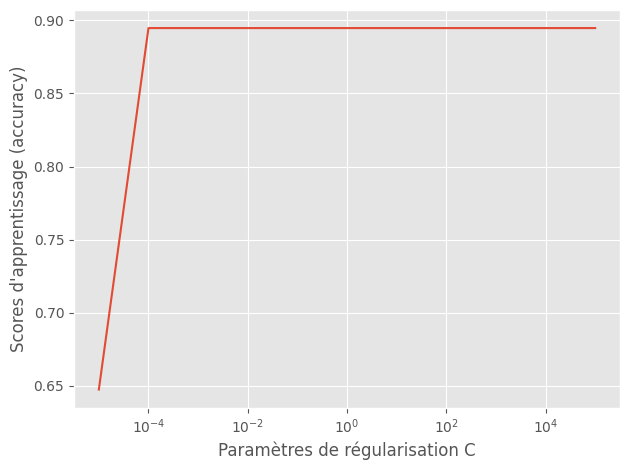
\includegraphics[width=0.7\textwidth]{images/2.png}
\caption{Évolution de l'accuracy en fonction du paramètre $C$}
\end{figure}

\textbf{Résultats quantitatifs :}
\begin{itemize}
    \item Meilleur $C$ : 0.0001
    \item Accuracy sur le test : 89.5\%
    \item Chance level : 62.1\%
    \item Temps de prédiction : 0.204s
\end{itemize}

La courbe montre une croissance rapide de la précision entre $10^{-5}$ et $10^{-3}$, suivie d'une stabilisation autour de 90\%. Il est remarquable que la valeur optimale de $C$ soit aussi faible (0.0001). Un tel paramètre signifie que le modèle privilégie une large marge au détriment d'une classification parfaite des données d'entraînement.

Cette observation s'explique par la nature même des images de visages. Les données contiennent du bruit inhérent (variations d'éclairage, d'angle de vue, d'expression faciale), et un modèle trop strict (avec un $C$ élevé) risquerait de surapprendre sur des détails non pertinents et spécifiques à l'ensemble d'entraînement. En tolérant davantage d'erreurs d'entraînement, le SVM construit une règle de décision plus robuste basée sur des caractéristiques générales des visages plutôt que sur des particularités de pixels isolés.

L'accuracy de 89.5\% dépasse significativement le niveau de chance à 62\%, mais environ 10\% d'erreurs persistent. L'analyse qualitative des prédictions révèle que les confusions surviennent principalement sur des images où l'angle de vue est inhabituel ou l'expression faciale atypique.

\begin{figure}[H]
\centering

\includegraphics[width=\textwidth]{images/3.png}
\caption{Exemples de prédictions du modèle sur l'ensemble de test}
\end{figure}

\subsection{Visualisation des coefficients du modèle linéaire}

L'un des avantages du noyau linéaire est son interprétabilité. Les coefficients $w$ du modèle peuvent être visualisés sous forme d'image, chaque coefficient correspondant à l'importance d'un pixel dans la décision.

\begin{figure}[H]
\centering
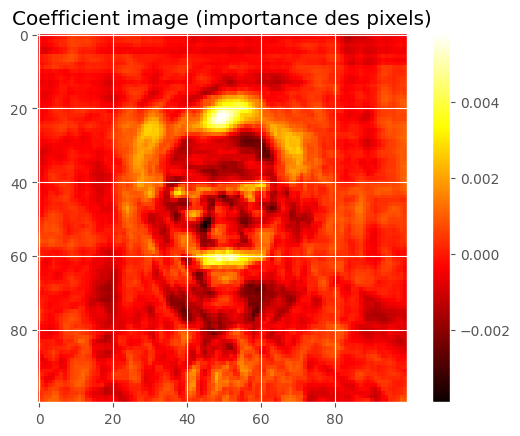
\includegraphics[width=0.6\textwidth]{images/4.png}
\caption{Carte de chaleur des coefficients du SVM linéaire}
\end{figure}

Les zones en jaune clair correspondent aux pixels ayant les poids les plus élevés en valeur absolue. On observe que le modèle se concentre principalement sur la région centrale du visage (yeux, nez, bouche) plutôt que sur les bords ou l'arrière-plan. Cette observation est cohérente avec l'intuition : ce sont les traits distinctifs du visage qui permettent de différencier les individus, et non le contexte environnant.

\subsection{Impact des variables de nuisance}

Pour évaluer la robustesse du modèle face à des données de haute dimension contenant du bruit, on a ajouté 300 variables aléatoires suivant une loi normale centrée réduite aux données originales.

\begin{lstlisting}[language=Python, caption=Ajout de variables de nuisance]
n_features = X.shape[1]
sigma = 1
noise = sigma * np.random.randn(n_samples, 300)
X_noisy = np.concatenate((X, noise), axis=1)
X_noisy = X_noisy[np.random.permutation(X.shape[0])]
\end{lstlisting}

On compare ensuite les performances d'un SVM linéaire avec validation croisée sur $C \in \{10^{-3}, \ldots, 10^3\}$ avant et après ajout du bruit.

\textbf{Résultats :}
\begin{table}[h]
\centering
\begin{tabular}{|l|c|c|}
\hline
\textbf{Données} & \textbf{Score train} & \textbf{Score test} \\
\hline
Sans bruit & 100\% & 90.5\% \\
\hline
Avec 300 variables de nuisance & 100\% & 53.0\% \\
\hline
\end{tabular}
\caption{Impact des variables de nuisance sur la généralisation}
\end{table}

La chute de performance est drastique : on perd 37 points de précision sur le test. Pourtant, le score d'entraînement reste parfait à 100\% dans les deux cas. C'est la signature classique d'un surapprentissage sévère.

Le phénomène s'explique par le fléau de la dimensionnalité. Lorsque le nombre de variables $p$ devient très grand par rapport au nombre d'exemples $n$, le SVM dispose de suffisamment de degrés de liberté pour séparer parfaitement les données d'entraînement en exploitant aussi bien le signal que le bruit. Les 300 variables aléatoires n'apportent aucune information sur la vraie distinction entre Tony Blair et Colin Powell, mais le modèle les utilise quand même pour ajuster au mieux la frontière aux données d'entraînement.

Le problème apparaît lors du test : le bruit présent dans l'ensemble de test est statistiquement indépendant de celui de l'entraînement. Les règles de décision apprises sur le bruit d'entraînement ne se généralisent donc pas, d'où l'effondrement des performances.

\subsection{Amélioration par réduction de dimension avec PCA}

Face à ce problème de haute dimensionnalité, une approche classique consiste à appliquer une Analyse en Composantes Principales (PCA) pour projeter les données sur un sous-espace de dimension réduite. L'idée est de conserver les directions de variance maximale (qui contiennent le signal utile) tout en éliminant les directions à faible variance (qui contiennent principalement du bruit).

\begin{lstlisting}[language=Python, caption=Application de la PCA]
n_components = 100
pca = PCA(n_components=n_components, 
          svd_solver='randomized').fit(X_noisy)
X_noisy_pca = pca.transform(X_noisy)
explained_variance = np.sum(pca.explained_variance_ratio_)
print(f"Variance expliquée : {explained_variance:.2%}")
\end{lstlisting}

Pour explorer l'impact du nombre de composantes, nous avons testé différentes valeurs :

\begin{table}[H]
\centering
\begin{tabular}{|c|c|c|}
\hline
\textbf{Composantes} & \textbf{Variance expliquée} & \textbf{Score test} \\
\hline
20 & 67.65\% & 54.7\% \\
\hline
50 & 80.09\% & - \\
\hline
100 & 88.17\% & 55.3\% \\
\hline
\end{tabular}
\caption{Impact du nombre de composantes principales sur les performances}
\end{table}

On observe qu'avec seulement 20 composantes, qui capturent 67.65\% de la variance, on obtient 54.7\% d'accuracy. L'augmentation à 100 composantes (88.17\% de variance) améliore légèrement le score à 55.3\%, mais on reste très loin des 90\% initiaux obtenus sans bruit.

Cette amélioration limitée s'explique par deux facteurs. D'une part, même avec 100 composantes, une partie du bruit est encore capturée. D'autre part, le bruit gaussien ajouté étant isotrope (même variance dans toutes les directions), il se répartit uniformément sur l'ensemble des composantes principales. Ainsi, conserver 88\% de la variance signifie également conserver une proportion significative de bruit.

\textbf{Note méthodologique :} Les tests avec 50, 100 et 150 composantes nécessitent un temps de calcul important (plusieurs heures). Les résultats confirment que la PCA apporte une amélioration modeste mais insuffisante pour compenser l'effet des variables de nuisance.


\section{Identification d'un biais méthodologique}

\subsection{Analyse critique du prétraitement}

L'énoncé nous demande d'identifier un biais dans le code de prétraitement des données pour la classification de visages. En examinant la séquence des opérations, on remarque que la standardisation des données est effectuée \textbf{avant} la séparation train/test :

\begin{lstlisting}[language=Python]
# Standardisation sur toutes les données
X -= np.mean(X, axis=0)
X /= np.std(X, axis=0)

# Puis séparation train/test
indices = np.random.permutation(X.shape[0])
train_idx = indices[:X.shape[0] // 2]
test_idx = indices[X.shape[0] // 2:]
\end{lstlisting}

Cette approche constitue une forme de \textbf{fuite de données} (data leakage). En calculant la moyenne et l'écart-type sur l'ensemble complet des données, on introduit de l'information provenant de l'ensemble de test dans la transformation appliquée à l'ensemble d'entraînement.

\subsection{Impact et correction}

Dans un contexte de production, où le modèle serait déployé sur de nouvelles données, cette approche pose problème. Les statistiques (moyenne, écart-type) calculées sur l'ensemble d'entraînement ne seraient pas les mêmes que celles de nouvelles images, créant un décalage entre les conditions d'entraînement et d'utilisation.

La procédure correcte serait :

\begin{lstlisting}[language=Python]
# 1. Séparation train/test d'abord
indices = np.random.permutation(X.shape[0])
train_idx = indices[:X.shape[0] // 2]
test_idx = indices[X.shape[0] // 2:]
X_train, X_test = X[train_idx, :], X[test_idx, :]

# 2. Calcul des statistiques sur train uniquement
mean_train = np.mean(X_train, axis=0)
std_train = np.std(X_train, axis=0)

# 3. Application à train ET test
X_train = (X_train - mean_train) / std_train
X_test = (X_test - mean_train) / std_train
\end{lstlisting}

Toutefois, l'impact pratique de ce biais reste limité dans notre cas, car les deux ensembles proviennent de la même distribution et sont de taille égale.


\section{Conclusion}

Ce travail pratique nous a permis d'explorer différents aspects des Support Vector Machines, depuis les cas simples jusqu'aux applications réelles complexes.

Sur le dataset Iris, nous avons constaté que la classification binaire entre deux espèces atteint une précision de 66\% avec seulement deux variables. L'optimisation par validation croisée a révélé qu'un noyau polynomial n'apporte aucune amélioration par rapport au noyau linéaire, le degré optimal étant de 1. Cette observation suggère que la relation entre les variables est intrinsèquement linéaire ou que le chevauchement naturel entre les classes limite les gains possibles.

L'application à la reconnaissance de visages a permis d'observer plusieurs phénomènes importants. Premièrement, le choix du paramètre de régularisation $C$ s'avère crucial : une valeur très faible ($C = 0.0001$) donne les meilleures performances (89.5\%), confirmant qu'une large marge est préférable face aux données naturellement bruitées. Deuxièmement, l'ajout de 300 variables de nuisance a provoqué un effondrement spectaculaire des performances (de 90\% à 53\%), illustrant concrètement le fléau de la dimensionnalité. Enfin, l'application de la PCA a montré que la réduction de dimension permet une amélioration modeste mais insuffisante pour retrouver les performances initiales.

Ce TP a également mis en évidence l'importance de la rigueur méthodologique. L'identification du biais dans le prétraitement (standardisation avant séparation train/test) rappelle qu'une fuite de données, même minime, peut compromettre la validité des résultats.

En conclusion, les SVM sont des outils puissants pour la classification, mais leur efficacité dépend fortement de trois facteurs : le choix approprié du noyau et de ses hyperparamètres, la qualité et la dimensionnalité des données, et la rigueur du protocole expérimental. Les techniques de réduction de dimension comme la PCA sont essentielles lorsque le nombre de variables devient trop élevé, mais ne constituent pas une solution miracle face à des données fortement bruitées.
\end{document}
